\documentclass[12pt]{article}
\usepackage{amsmath, amsfonts, amssymb}
\usepackage{mathtools}
\usepackage{datetime}
\usepackage{interval}
\usepackage{subfig}
\usepackage{graphicx}
\usepackage{float}
\usepackage{geometry}
\usepackage[makeroom]{cancel}

\geometry{a4paper,scale=0.78}
\DeclarePairedDelimiter\floor{\lfloor}{\rfloor}
\setlength{\parskip}{1em}
\title{MATH3320 Project Report\\Topic: Image Compression}
\author{ZHANG Xinfang 1155141566\\ZHANG Yifan 1155141570}
\newdate{date}{08}{11}{2021}
\date{\displaydate{date}}

\begin{document}   
\maketitle
% \newpage
% Part 1: introduction

\section*{1.\quad Introduction}
\begin{flushleft}
In recent years, with the rapid developement in technology, multimedia product 
of digital information grows increasingly fast, which requires a large memory space 
and sufficient bandwidth in the storage and transmission process. 
Therefore, data compression becomes extremely vital for reducing the data 
redundancy to save more hardware space and transmission bandwidth. 

Image compression is the process of removing redundant and irrelevant information, 
and efficiently encoding or reverting what remains without affecting or degrading its quality. 
The objective of image compression is to store or transmit data in an efficient form
and to reduce the storage quantity as much as possible.

One useful techniques in image compression is to decompose an image into linear combination 
of elementary images with specific properties. By truncating some less important components 
in the image decomposition, we can compress an image to reduce the image size 
and achieve transform coding. 

In this paper, we will discuss some useful image decomposition methods, demonstrate the 
applications of these decomsotion methods for image compression and analyze their advantages,
disadvantages and applicability.
\end{flushleft}
\newpage
% Part2: Method
    % 1) definition + formula
    % 2) proof + error computation
    % 3) code + example

\section*{2.\quad Image Compression Models}
\subsection*{2.1\quad Singular Value Decomposition (SVD)}
\subsubsection*{2.1.1 \quad Definition}
Every $m\times n$ image $g$ has a singular value decomposition.\\
For any $g \in M_{m \times n}$, the singular value decomposition (SVD) of $g$ is
 a matrix factorization give by \\
 \centerline{$g = U \Sigma V^T$}\\
 with $U \in M_{m \times m}$ and $V \in M_{n \times n}$ both unitary, and $\Sigma \in 
 \mathbb{R}^{m \times n}$ is a diagonal matrix with diagonal elements 
 $\sigma_1 \geq\sigma_2\geq\cdots\geq\sigma_r > 0$ with r $\leq$ min ($m$,$n$). 
The diagonal elements are called singular values. 
Then we have\\
\centerline{$g = U \Sigma V^T = \sum\limits_{i=1}^{r}\sigma_i \vec{u_i}\vec{v_i}^T$},
where $\vec{u_i}\vec{v_i}^T$ is called the eigenimages of g under SVD.

\noindent
The most interesting part of SVD methods is that the data arrange in such a way that the most 
important data is stored on the top, which corresponds to the top eigenvalues and eigenimages.

\subsubsection*{2.1.2 \quad Application}
SVD can be applied for image compression, by removing terms (eigenimages) associated to small singular values.
We will show examples of image compression using SVD, so-called 'rank-k approximation'. The whole implementation of 
this report is done using Python. For simplicity, we convert all images into grayscale images first. The packages and 
grayscalized process are as follows:
\begin{figure}[H]
    \centering
    \subfloat[Import packages]{
        \label{ref_label1}
        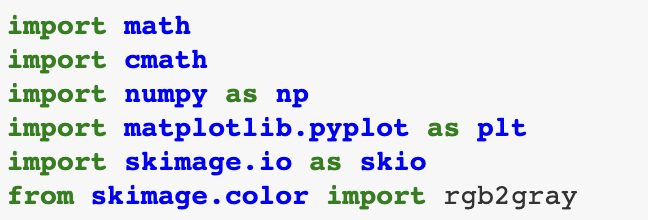
\includegraphics[width=0.5\textwidth]{library.png}
        }
    \subfloat[Read and convert images]{
        \label{ref_label2}
        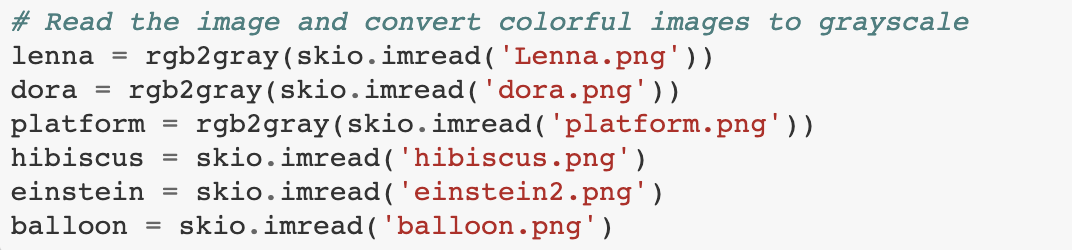
\includegraphics[width=0.5\textwidth]{rgb2gray.png}
        }\\
    \caption{Packages and pre-processing}
\end{figure}
\begin{flushleft}
Here is the results for different rank-k. (\# of singular values = 512)  
\end{flushleft}
\begin{figure}[H]
    \centering
    \subfloat[k = 10]{
        \label{ref_label1}
        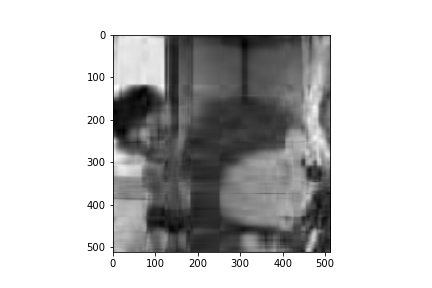
\includegraphics[width=0.5\textwidth]{dora_10.png}
        }
    \subfloat[k = 40]{
        \label{ref_label2}
        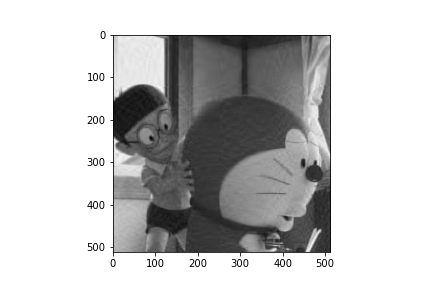
\includegraphics[width=0.5\textwidth]{dora_40.png}
        }\\
    \subfloat[k = 100]{
        \label{ref_label2}
        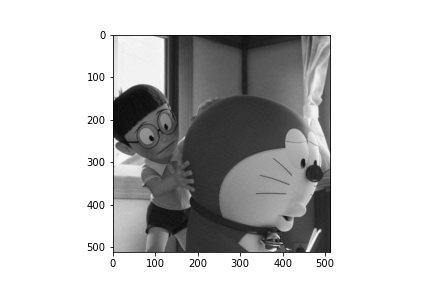
\includegraphics[width=0.5\textwidth]{dora_100.png}
        }
    \subfloat[Original]{
        \label{ref_label2}
        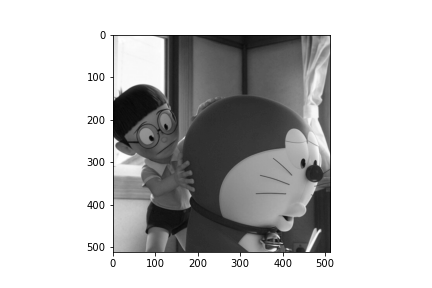
\includegraphics[width=0.5\textwidth]{dora_orig.png}
        }
    \caption{Doraemon and its compressed images using SVD}
    \label{ref_label_overall}
\end{figure}
\begin{flushleft}
Since the weightings of eigenimages depend on corresponding singular values, the larger the singular value is,
the more important the eigen-image is. Hence, we consider ignoring singular values which are less than 0.5\% of the 
largest singular value automatically so that the image can be compressed without losing too much information and influcing
the image quality. Our code and result are as follows:\\
\end{flushleft}
\pagebreak
Code:
\begin{figure}[H]
    \centering
    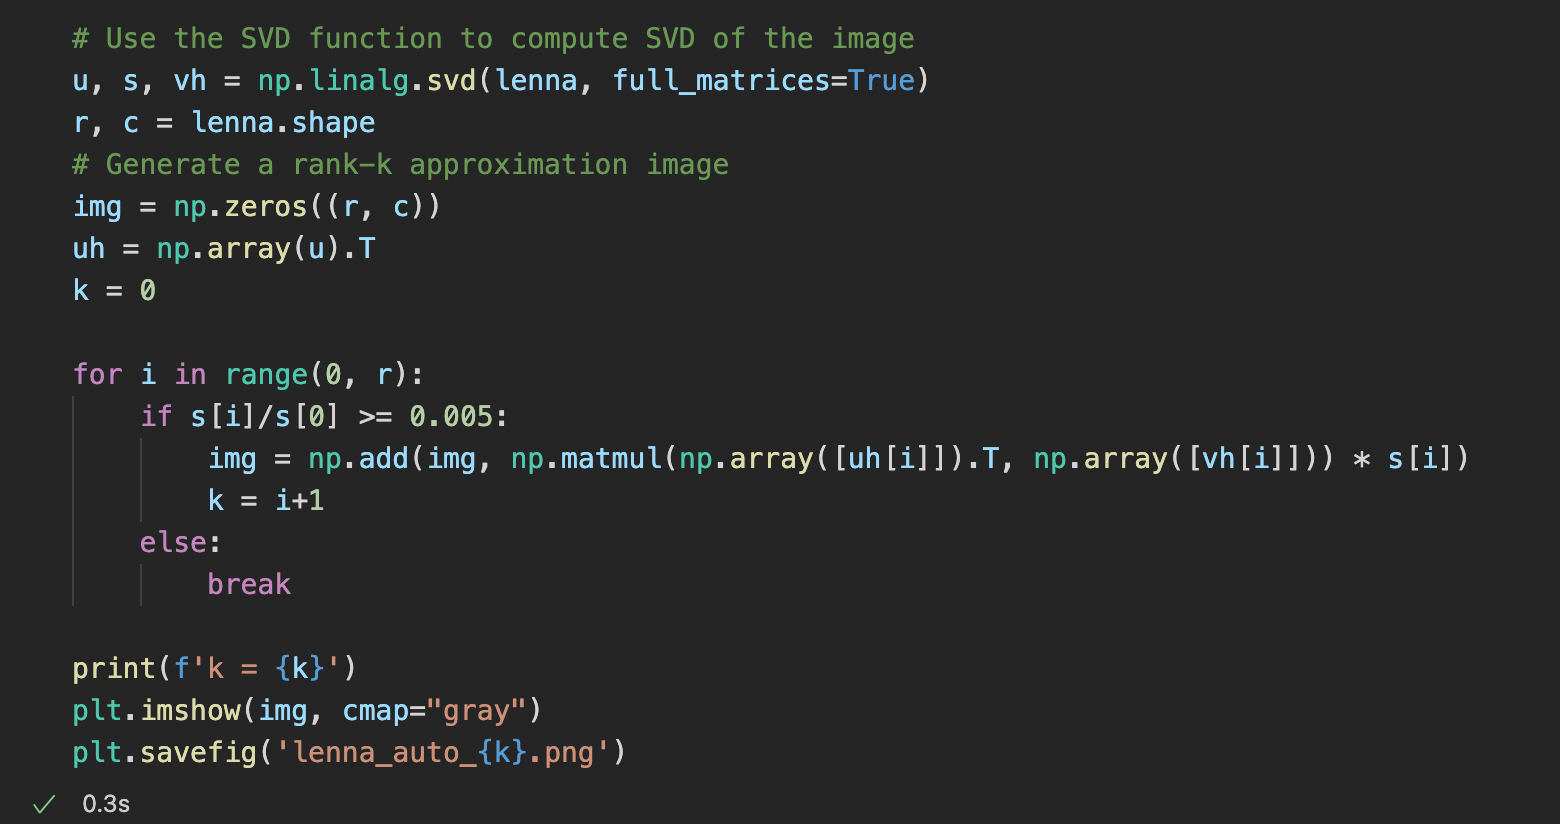
\includegraphics[width=1\textwidth]{SVD_code.png}
    \caption{SVD Algorithm}
\end{figure}
\begin{flushleft}
Results: 
\end{flushleft}
\begin{figure}[H]
    \centering
    \subfloat[Algorithm with k = 86]{
        \label{ref_label2}
        \includegraphics[width=0.5\textwidth]{dora_auto_{k}.png}
        }
    \subfloat[Original]{
        \label{ref_label2}
        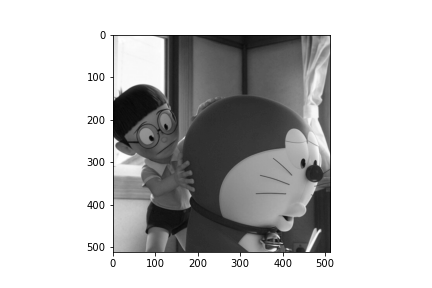
\includegraphics[width=0.5\textwidth]{dora_orig.png}
        }
    \caption{SVD algorithm results}
    \label{ref_label_overall}
\end{figure}
\begin{flushleft}
Now we use the same algorithm to test another image called 'Lenna'. The comparison between 
SVD compressed images and the original image are as follows: (\# of singular values = 512)  
\end{flushleft}
\begin{figure}[H]
    \centering
    \subfloat[k = 20]{
        \label{ref_label1}
        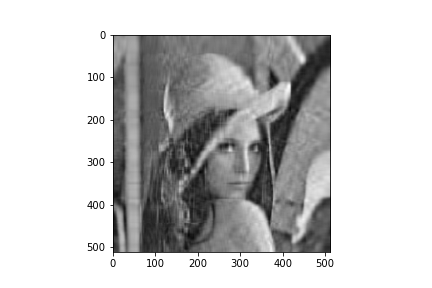
\includegraphics[width=0.5\textwidth]{lenna_20.png}
    }
    \subfloat[k = 50]{
        \label{ref_label2}
        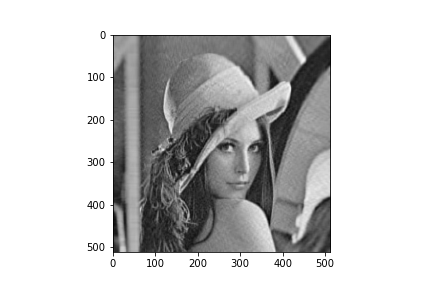
\includegraphics[width=0.5\textwidth]{lenna_50.png}
    }\\
    \subfloat[Algorithm with k = 107]{
        \label{ref_label2}
        \includegraphics[width=0.5\textwidth]{lenna_auto_{k}.png}
    }
    \subfloat[Original]{
        \label{ref_label2}
        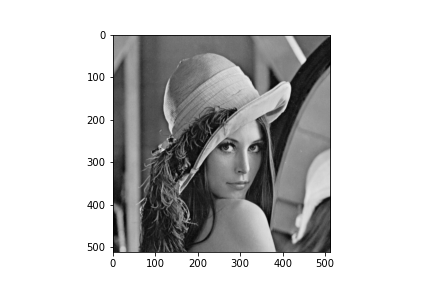
\includegraphics[width=0.5\textwidth]{lenna_orig.png}
    }
    \caption{Lenna and its compressed images using SVD}
    \label{ref_label_overall}
\end{figure}
\subsubsection*{2.1.3 \quad Error Analysis}
For any $k$ with $0\leq k \leq r$, we define
\begin{equation*}
    g_k = \sum_{j=1}^{k}\sigma_j \vec{u_j}\vec{v_j}^T,
\end{equation*} 
where $g_k$ is called a rank-k approximation of $g$.
This low rank matrix approximation can be applied to image compression. 
\begin{flushleft}
Here we apply Frobenius norm to compute the error of approximation:\\
\end{flushleft}
Let $f=\sum\limits_{j=1}^{r}\sigma_j \vec{u_j}\vec{v_j}^T$  be the SVD of an $M \times N$ image $f$.
For any $k$ with $k<r$, and $f_k = \sum\limits_{j=1}^{k}\sigma_j \vec{u_j}\vec{v_j}^T$, we have
\begin{equation*}
    {\| f-f_k\|}_F^2 = \sum_{j=k+1}^{r}\sigma_j^2
\end{equation*}
\textit{Proof}: Let $f=\sum\limits_{j=1}^{r}\sigma_j \vec{u_j}\vec{v_j}^T$.\\
Approximate $f$ by $f_k$ with $k<r$ where $f_k = \sum\limits_{j=1}^{k}\sigma_j \vec{u_j}\vec{v_j}^T$\\
Define the error of the approximation by $D\equiv f-f_k = \sum\limits_{j=k+1}^{r}\sigma_j \vec{u_j}\vec{v_j}^T \in M_{m\times n}$
Then the $m$-th row, $n$-th column entry of $D$ is given by
\begin{equation*}
    D_{mn} = \sum_{j=k+1}^{r}\sigma_j^2u_{im}v_{in}
\end{equation*}
where $\vec{u_i}= \left( \begin{array}{c} u_{i1} \\ \vdots \\ u_{iM} \end{array} \right)$,
$\vec{v_i}= \left(\begin{array}{c} v_{i1} \\ \vdots \\ v_{iN} \end{array} \right)$. Then,
\begin{flalign*}
        {\| D \|}_F^2 &= \sum\limits_{m} \sum\limits_{n} D_{mn}^2 &\\
        &= \sum\limits_{m}\sum\limits_{n}\left(\sum\limits_{i=k+1}^{r}\sigma_i^2u_{im}^2v_{in}^2 + 2\sum\limits_{i=k+1}^{r}\sum\limits_{\substack{j=k+1\\j\neq i}}^{r} \sigma_i\sigma_j u_{im}v_{in}u_{jm}v_{jn}\right) &\\
        &= \sum\limits_{i=k+1}^{r}\sigma_i^2 \cancelto{1}{\sum\limits_{m}u_{im}^2} \cancelto{1}{\sum\limits_{n}v_{in}^2} + 2\sum\limits_{\substack{j=k+1\\j\neq i}}^{r} \sigma_i\sigma_j\cancelto{0}{\sum\limits_{m}u_{im}u_{jm}}\cancelto{0}{\sum\limits_{n}v_{in}v_{jn}} &\\ 
        &= \sum\limits_{i=k+1}^{r}\sigma_i^2 &
\end{flalign*}
Therefore, we prove that\\
\textbf{ Sum of square error of the approximation = Sum of omitted eigenvalues}.


\subsection*{2.2\quad Haar Transform and Walsh Transform}

\subsubsection*{2.2.1 \quad Haar Function and Haar Transform}
Haar function:
    \begin{equation*}
            H_m(t) = H_{2^p+n}(t) = \begin{cases} 
                2^{\frac{p}{2}} & \text{if $\frac{n}{2^p} \leq t \leq \frac{n+0.5}{2^p}$} \\  
                -2^{\frac{p}{2}} & \text{if $\frac{n+0.5}{2^p} \leq t \leq \frac{n+1}{2^p}$} \\  
                0 & \text{elsewhere}  
                \end{cases}
    \end{equation*}
\hspace*{1cm} where $p$ = 1, 2, \ldots; $n$ = 0, 1, 2, \ldots, $2^{p-1}$
\begin{flushleft}
Based on the Haar function, Haar Transform of $N\times N$ image is defined as follow.\\
Let $H(k,i) \equiv H_{k}\left(\frac{i}{N}\right)$ where $k,i$ = 0, 1, 2, \ldots, $N$-1 \\
We obtain the Haar Transfrom matrix:
\begin{equation*}
 \tilde{H} \equiv\frac{1}{\sqrt{N}}H, \quad H \equiv(H (k,i))_{0\leqslant k,i \leqslant N-1}
\end{equation*}
The Haar Transfrom of $f \in M_{n\times n}$ is defined as:
\begin{equation*}
    g = \tilde{H}f\tilde{H}^T
\end{equation*}
\end{flushleft} 

\subsubsection*{2.2.2 \quad Walsh Function and Walsh Transform}
Walsh function is defined recursively as follows: 
\begin{equation*}
    W_{2j+q}(t) = (-1)^{\floor*{\frac{j}{2}}+q} \{W_j(2t)+(-1)^{j+q}W_j(2t-1)\}
\end{equation*} 
where $q$ = 0 or 1; $j$ = 0, 1, 2, \dots and $W_0(t) = \begin{cases}
        1 & \text{if $0 \leq t < 1$}\\
        0 & \text{elsewhere}
    \end{cases}$\\
\begin{flushleft}
Based on Walsh function, Walsh Transfrom of $N\times N$ image is defined as follow.\\
Let $W(k,i) \equiv H_{k}\left(\frac{i}{N}\right)$ where $k,i$ = 0, 1, 2, \ldots, $N$-1 \\
We obtain the Walsh Transfrom matrix:
\begin{equation*}
 \tilde{W} \equiv\frac{1}{\sqrt{N}}W, \quad W \equiv(W (k,i))_{0\leqslant k,i \leqslant N-1}
\end{equation*}
The Walsh Transfrom of $f \in M_{n\times n}$ is defined as:
\begin{equation*}
    g = \tilde{W}f\tilde{W}^T
\end{equation*}
\end{flushleft} 

\subsubsection*{2.2.3 \quad Application}
According to the definition in last subsection, the transformation codes and transformed images are implemented as follows:
\begin{flushleft}
(a) Haar Transform 

Code:
\end{flushleft}

\begin{figure}[H]
    \centering
    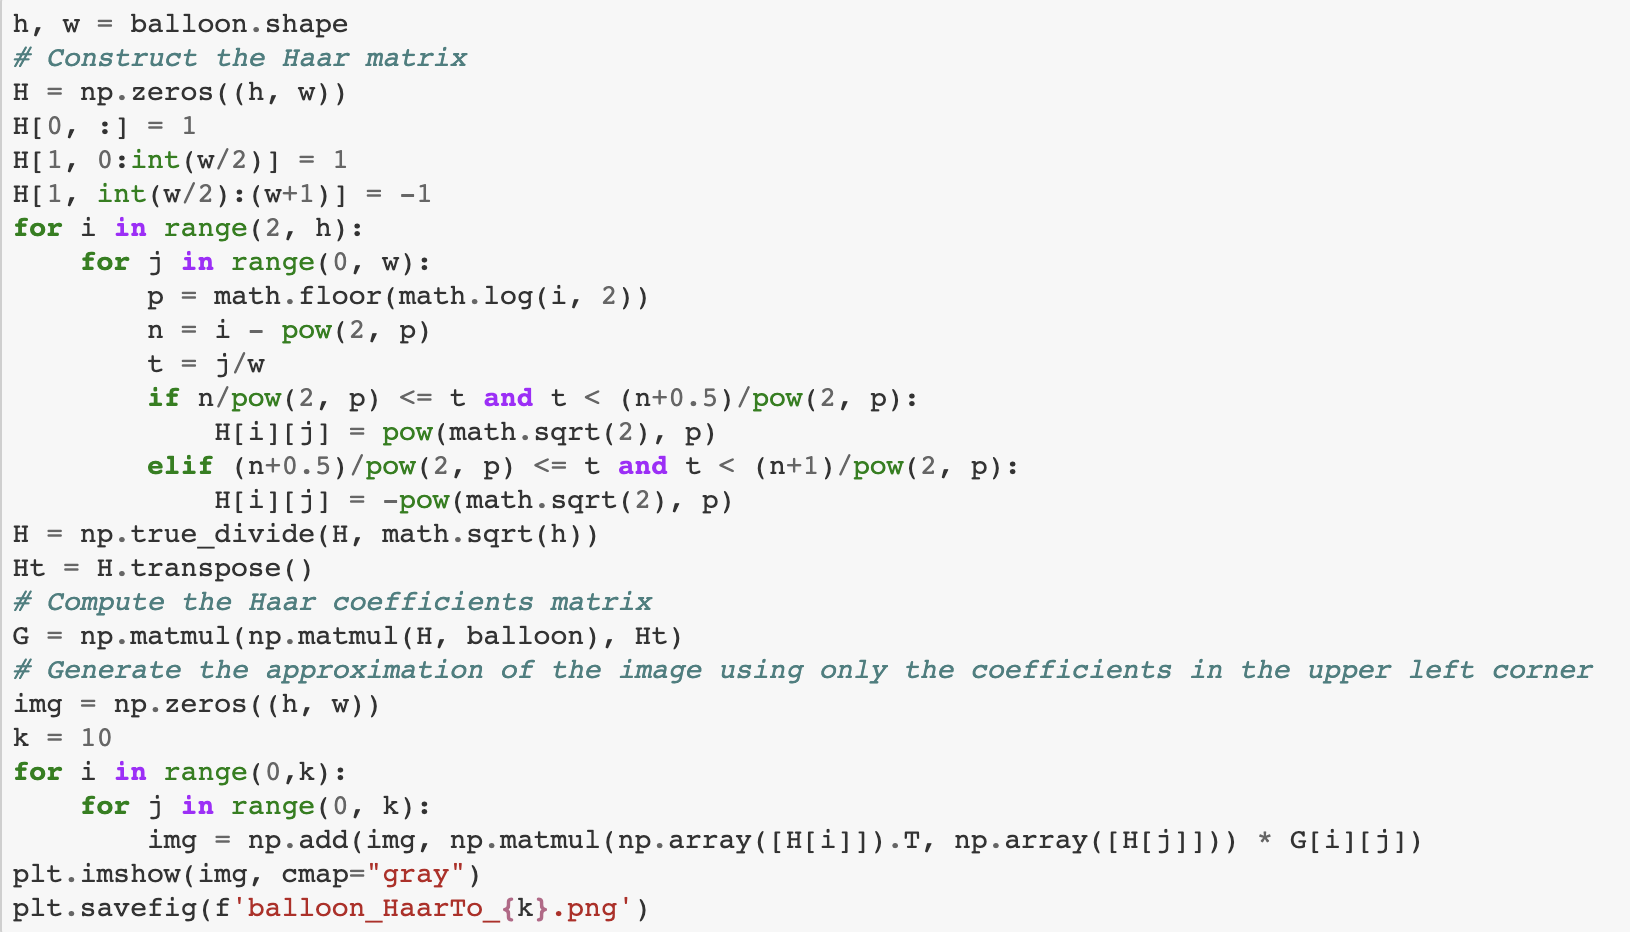
\includegraphics[width=1\textwidth]{haar_code.png}
    \caption{Haar Transform Codes}
\end{figure}
\begin{flushleft}
Results:

In forllowing figures, we keep upper left corner Haar coefficients in Haar transform matrix up to  $2 \times 2$, 
$3 \times 3$, $4 \times 4$, \dots respectively.
(Size of this 'balloon' image = $128 \times 128$)
\end{flushleft}
\begin{figure}[H]
    \centering
    \subfloat[Haar to 2]{
        \label{ref_label1}
        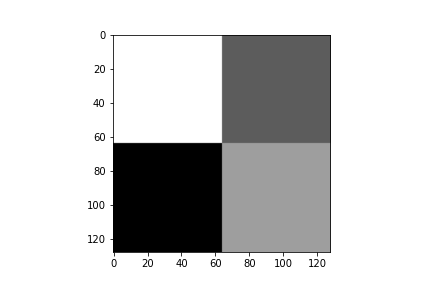
\includegraphics[width=0.3\textwidth]{balloon_HaarTo_2.png}
        }
    \subfloat[Haar to 3]{
        \label{ref_label2}
        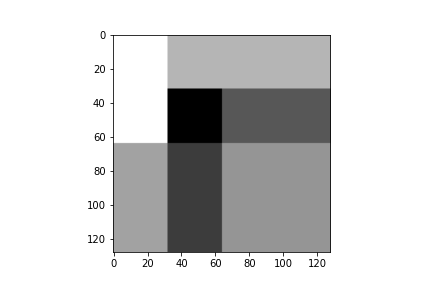
\includegraphics[width=0.3\textwidth]{balloon_HaarTo_3.png}
        }
    \subfloat[Haar to 4]{
        \label{ref_label2}
        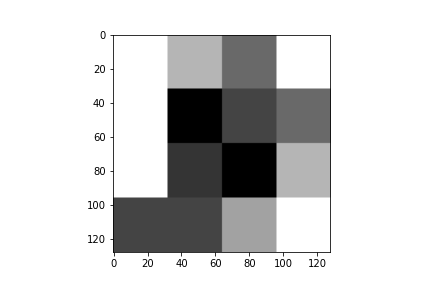
\includegraphics[width=0.3\textwidth]{balloon_HaarTo_4.png}
        }\\
    \subfloat[Haar to 5]{
        \label{ref_label2}
        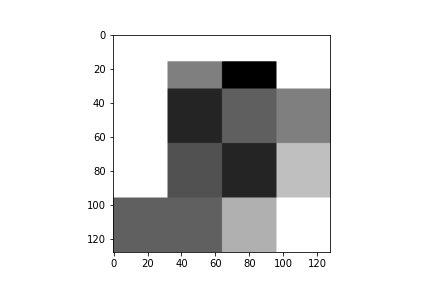
\includegraphics[width=0.3\textwidth]{balloon_HaarTo_5.png}
        }
    \subfloat[Haar to 6]{
        \label{ref_label2}
        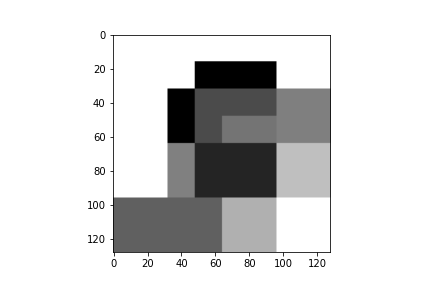
\includegraphics[width=0.3\textwidth]{balloon_HaarTo_6.png}
        }
    \subfloat[Haar to 7]{
        \label{ref_label2}
        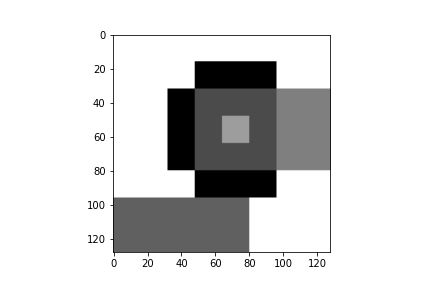
\includegraphics[width=0.3\textwidth]{balloon_HaarTo_7.png}
        }
    \caption{Balloon and its compressed images using Haar Transform}
    \label{ref_label_overall}
\end{figure}
\begin{figure}[H]
    \centering
    \subfloat[Haar to 10]{
        \label{ref_label1}
        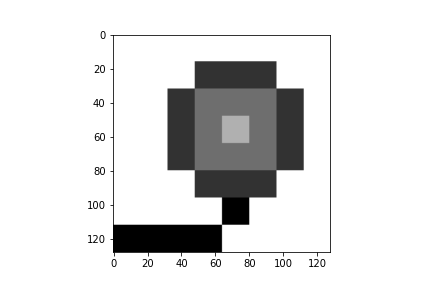
\includegraphics[width=0.5\textwidth]{balloon_HaarTo_10.png}
        }
    \subfloat[Original]{
        \label{ref_label2}
        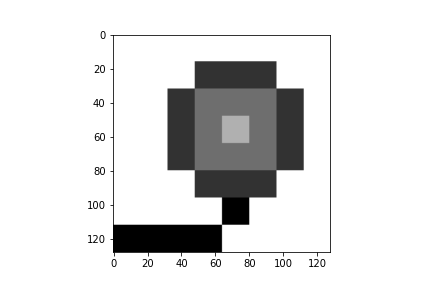
\includegraphics[width=0.5\textwidth]{balloon_orig.png}
        }
    \caption{Haar Compression VS Original Image}
    \label{ref_label_overall}
\end{figure}
\begin{flushleft}
It is obvious that 'Haar to 10' has already achieved a good performance compared to the original image size.

(b) Walsh Transform

The implementation logic for Walsh Transform is similar to that for Haar Transform. Therefore, we only put the 
sample images of different size of upper left corner of Walsh coefficients here.
\end{flushleft}
\begin{figure}[H]
    \centering
    \subfloat[Walsh to 2]{
        \label{ref_label1}
        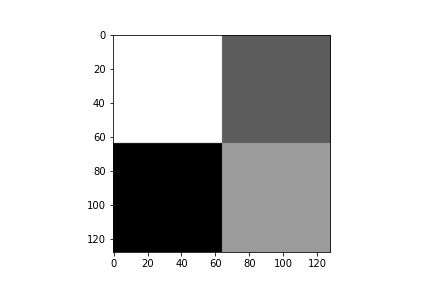
\includegraphics[width=0.3\textwidth]{balloon_walshTo2.png}
        }
    \subfloat[Walsh to 3]{
        \label{ref_label2}
        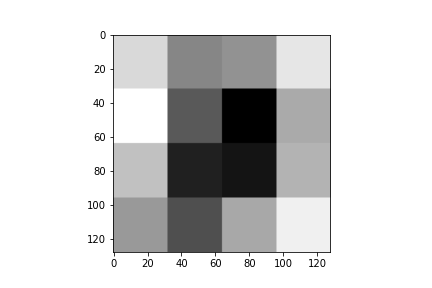
\includegraphics[width=0.3\textwidth]{balloon_walshTo3.png}
        }
    \subfloat[Walsh to 4]{
        \label{ref_label2}
        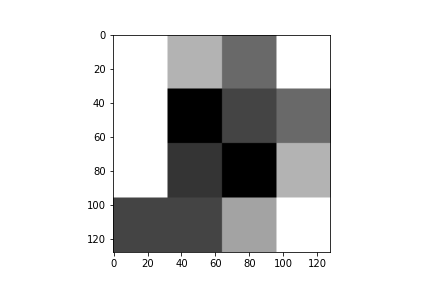
\includegraphics[width=0.3\textwidth]{balloon_walshTo4.png}
        }\\
    \subfloat[Walsh to 5]{
        \label{ref_label2}
        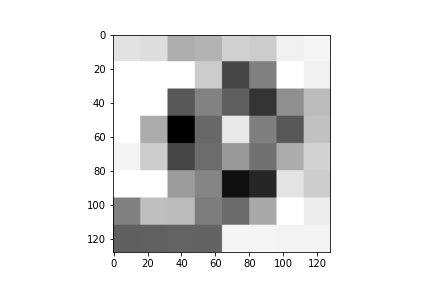
\includegraphics[width=0.3\textwidth]{balloon_walshTo5.png}
        }
    \subfloat[Walsh to 6]{
        \label{ref_label2}
        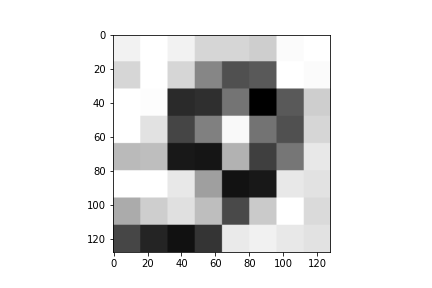
\includegraphics[width=0.3\textwidth]{balloon_walshTo6.png}
        }
    \subfloat[Walsh to 7]{
        \label{ref_label2}
        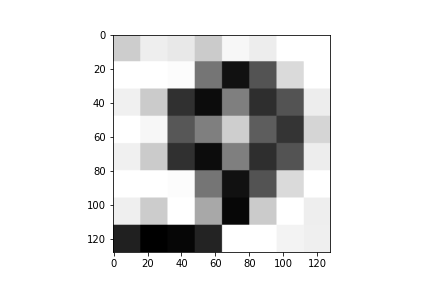
\includegraphics[width=0.3\textwidth]{balloon_walshTo7.png}
        }
    \caption{Balloon and its compressed images using Walsh Transform}
    \label{ref_label_overall}
\end{figure}

\subsection*{2.3\quad Discrete Fourier Transform (DFT)}

\subsubsection*{2.3.1\quad Definition}
The 2D \textbf{discrete Fourier Transform (DFT)} of a $M\times N$ image $g = (g(k,l)_{k,l})$ 
where $k$ = 0,1,\ldots, $M$-1 and $l$ = 0,1,\ldots, $N$-1, is defined as 
\begin{equation*}
    \tilde{g}(m,n) = \frac{1}{MN}\sum_{k=0}^{M-1}\sum_{l=0}^{N-1}g(k,l)e^{-2\pi j(\frac{km}{M}+\frac{ln}{N})}
\end{equation*}
And the inverse discrete Fourier Transform is given by
\begin{equation*}
    g(p,q) = \sum_{m=0}^{M-1}\sum_{n=0}^{N-1}\tilde{g}(m,n)e^{2\pi j(\frac{pm}{M}+\frac{qn}{N})}
\end{equation*}
Define matrix $U=(U_{x\alpha})_{0\leqslant x,\alpha \leqslant N-1}\in M_{N\times N}(\mathbb{C})$
by $U_{x\alpha}=\frac{1}{N} e^{-2\pi j\frac{x\alpha}{N}}$, where $0\leqslant x,\alpha \leqslant N-1$\\
Then U is symmetric and 
\begin{equation*}
    \tilde{g} = UgU
\end{equation*}
Besides, we can prove that rows of $U$ are mutually orthogonal but not orthonormal.\\
Then we conclude that $UU^{\ast}=\frac{1}{N}I$

% remaining part of DFT will all be done by xff --<3
% U can start conclusion directly
% 筆芯芯
\subsubsection*{2.3.2\quad Application}
(a) Fast Fourier Transform Algorithm (FFT)

\begin{flushleft}
(b) Example

Code: 
\end{flushleft}

\begin{flushleft}
Results:
\end{flushleft}

\begin{flushleft}
(c) Even Discrete Cosine Transform (EDCT)
\end{flushleft}


% Part3: Result
    % Error, computation cost
    % (Ppt comparison chart???)
    % 說一說 為什麼? 哪種圖片更適合哪種方法? 方法的特點
    % dont ask me why, dont wanna open the pages again

\section*{3.\quad Conclusion}






\end{document}